\section{Introduction}
%•	Présentation du sujet et de son importance.
\subsection{Contexte et enjeux}
%Abord IOT
L'IoT\footnote{Internet des objets} a révolutionné de nombreux aspects de notre société: la santé, de l'agriculture à l'industrie 4.0, en passant par les transports et les communications.
Les \textbf{technologies embarquées et connectées} désignent l’ensemble des systèmes électroniques intégrés aux véhicules (voitures et motos) permettant d’améliorer la sécurité, le confort et la connectivité. Ces technologies incluent : les systèmes de communication, les capteurs, les caméras, les radars, les lidars, les systèmes d’aide à la conduite (ADAS) et les plateformes de gestion des données.\\
%enjeux -> sécurité routière
L’accidentalité routière en France reste un enjeu majeur de sécurité publique, avec des milliers d’accidents chaque année causant des pertes humaines et matérielles importantes. Malgré les avancées en matière de prévention et de réglementation, les comportements à risque et les conditions de circulation continuent d’alimenter cette problématique.
En France, il y a environ 2,3 à 2,5 millions de motards\cite{actiEouteNbMotardFr}, ce qui représente 2\%  du trafic.
Le document\cite{la_securite_routiere_accidentalite_2024} fournit des informations et des statistiques sur les accidents de la route. Les données définitives datent du 31 mai 2024.

\begin{figure}[h]
    \centering
    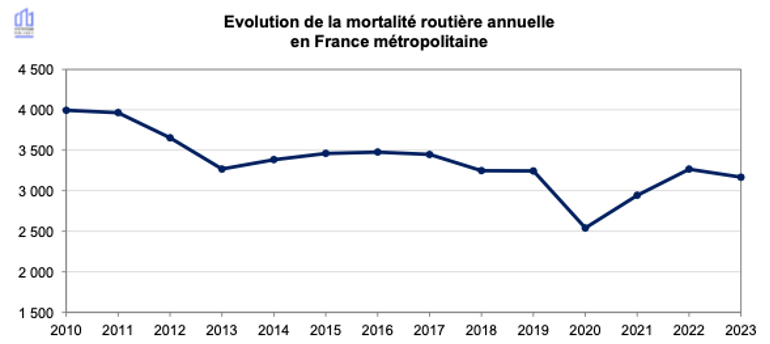
\includegraphics[width=0.7\textwidth]{images/evolution_mortalite_securite_routiere_france.png} 
    \caption{ONISR données relatives aux accidents corporels enregistrés par les forces de l'ordre en France métropolitaine.}
\end{figure}

Grâce au graphe précédent, on constate qu’il y a une diminution sensible du nombre d’accidents mortels sur la dernière décennie surtout entre 2011 et 2013. Différents paramètres expliquent cette évolution : nouvelles infrastructures routières, les dernières technologies de sécurité (casques, ABS…), les renforcements de la règlementation, mise en place de radars et nombreuses campagnes de sensibilisation… L’ensemble de ces éléments ont contribué à réduire la mortalité bien que chaque année, on enregistre, encore, autour de 3500 morts sur les routes tous véhicules confondus. 

\begin{figure}[h]
    \centering
    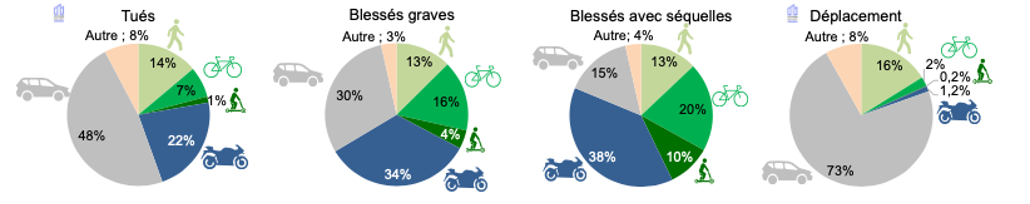
\includegraphics[width=0.7\textwidth]{images/camambert_accidents_differents_vehicules.png} 
    \caption{ONISR Données relatives aux accidents corporels enregistrés par les forces de l'ordre, en France métropolitaine.}
\end{figure}

En termes d’accidents corporels et de mortalité sur la route, les conducteurs de deux-roues sont les plus impactés. Le conducteur n’étant pas protégé par une carrosserie, il est plus vulnérable en cas d’accident. Le motard doit s’équiper de façon rigoureuse afin de limiter les blessures corporelles causées par le choc.\\
%enjeux -> technologies
C'est un défi majeur pour les autorités et les constructeurs de véhicules de trouver des solutions pour réduire le nombre d'accidents et améliorer la sécurité des usagers de la route, en particulier des motards. Les technologies IoT offrent des opportunités pour répondre à ces enjeux en améliorant la détection des obstacles, la perception environnementale, l'aide à la conduite et l'analyse des données pour une meilleure prise de décision.\\


\subsection{Définitions et concepts clés}
%••	IoT (Internet des Objets) appliqué aux transports.
Qu'est-ce que l'IoT ?\\
L'IoT est un réseau d’objets physiques connectés à Internet qui sont capables de collecter et d’échanger des données en temps réel. Ces objets peuvent être des capteurs, des appareils domestiques intelligents, des équipements industriels, des véhicules et bien plus encore. Ils font face à des défis et des enjeux importants comme l'exposition aux menaces de cyberattaques, l'uniformité des systèmes pour leur bon fonctionnement, la consommation d'énergie et enfin, le respect aux droits privés. \\
• \textbf{Les capteurs et caméras} : détectent les obstacles, surveillent l’environnement et assistent à la conduite (ex. : radars, lidars, caméras 360°). Selon dDruid\cite{capteur} un capteur IoT est un "composant électronique qui transforme les variations physiques ou environnementales en signaux électriques exploitables pour surveiller, contrôler ou interagir avec des systèmes connectés".
Les principaux types de capteurs d'IoT sont: les capteurs de température et d'humidité, les capteurs de mouvement et de présence, les capteurs de lumière et de luminosité, les capteurs de gaz et de qualité de l’airCapteurs de pression et de force et enfin les capteurs de proximité et de distance.
\begin{figure}[H]
    \centering
    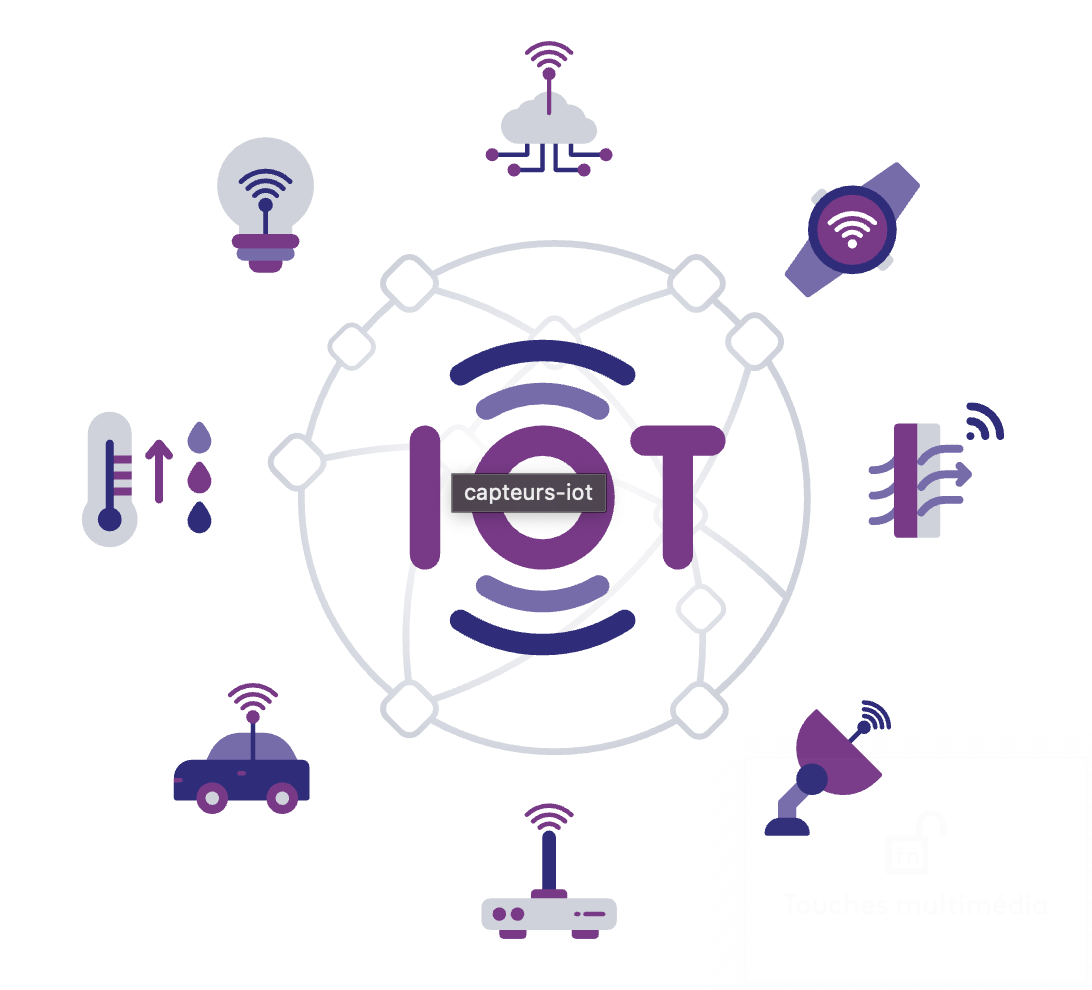
\includegraphics[width=0.5\textwidth]{images/capteur.png} 
    \caption{Intéraction des capteurs}
\end{figure}
Ils fonctionnent de manière autonome tout intégrant des réseaux connectés. Les éléments à identifier en premier lieu sont donc : leur taille, leur consommation d’énergie, leur capacité de traitement local, leur autonomie, leur capacité de communication.\\
• \textbf{Les systèmes d’aide à la conduite (ADAS)} : aident le conducteur en régulant la vitesse, le freinage d’urgence ou le maintien de trajectoire.\\
• \textbf{Les modules de connectivité (4G, 5G, Wi-Fi, Bluetooth)} : permettent l’échange de données en temps réel entre le véhicule et d’autres systèmes, comme les infrastructures routières ou les smartphones.\\
• \textbf{Les plateformes de gestion des données} : traitent les informations collectées pour fournir des services comme la navigation intelligente, l’alerte trafic ou la maintenance prédictive.\\
Ces technologies sont essentielles pour le développement des véhicules intelligents et autonomes, ainsi que pour renforcer la sécurité des motards, souvent plus vulnérables sur la route.\\
\vspace{0.5cm}

Les \textbf{communications V2V (e) et V2I (Vehicle-to-Infrastructure)} font partie des technologies de transport intelligent (ITS)\footnote{infrastructure technology services} qui permettent aux véhicules et aux infrastructures routières comme les feux de signalisation, les panneaux d’échanger des informations en temps réel.

\begin{figure}[H]
    \centering
    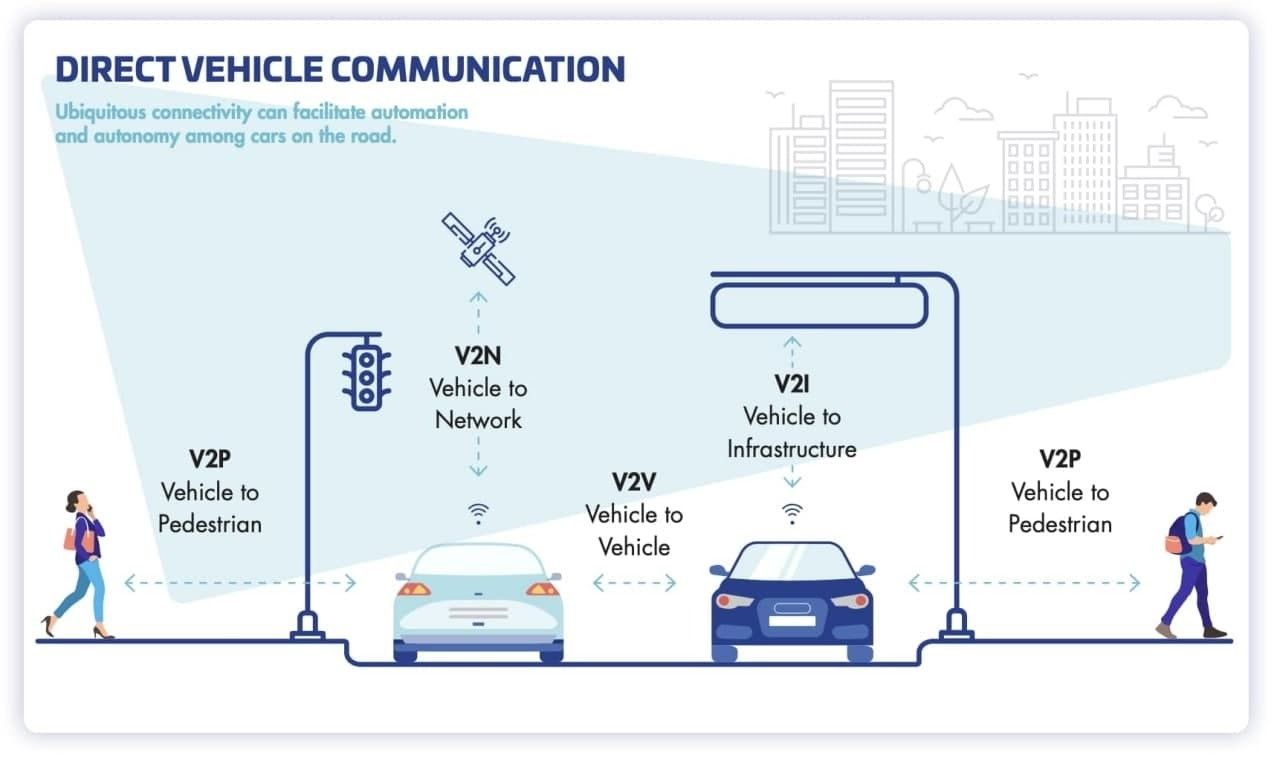
\includegraphics[width=0.7\textwidth]{images/schema_v2.png} 
    \caption{La communication V2X}
\end{figure}

Cette communication offre des mises à jour en temps réel sur les conditions de circulation, les accidents, la météo et la disponibilité des places de stationnement, améliorant ainsi la sécurité et l’efficacité des trajets\cite{joberty_blog}.\\
